\documentclass[11pt]{beamer}
\usepackage[utf8]{inputenc}
\usepackage[T1]{fontenc}
\usetheme{default}
%\usepackage{listings}
\usepackage{tikz}
\usetikzlibrary{overlay-beamer-styles}
\begin{document}



\begin{frame}[t]{Tree demo} % ================================================================
\begin{itemize}[<+->]
\item text1
\item text2
\end{itemize}

\begin{onlyenv}<+->
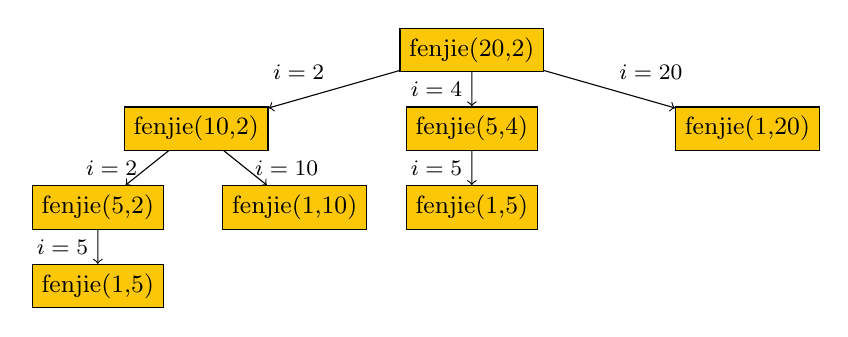
\begin{tikzpicture}[every node/.style={draw, fill={yellow!80!red}, font=\small},
                level distance=10mm,
                level 1/.style={sibling distance=3.5cm},
                level 2/.style={sibling distance=2.5cm}]]
\tikzset{nofill/.style={font=\footnotesize, fill=none, draw=none},
normalarr/.style={->}}

\node[visible on=<2->] at (5, 3.3) {fenjie(20,2)}
    child [normalarr,visible on=<3->] {node {fenjie(10,2)}
        child[visible on=<4->] {node {fenjie(5,2)}
            child[visible on=<5->]  {node{fenjie(1,5)} edge
            from parent node[nofill,left,visible on=<6->] {$i=5$}}
            edge from parent node[nofill,left,visible on=<7->] {$i=2$}
        }
        child[visible on=<8->] {node {fenjie(1,10)} edge from parent node[nofill,right] {$i=10$}}
        edge from parent node[nofill,above left] {$i=2$}
    }
    child[visible on=<9->,normalarr] {node {fenjie(5,4)}
        child {node {fenjie(1,5)} edge from parent node[nofill,left] {$i=5$}}
        edge from parent node[nofill,left] {$i=4$}
    }
    child[visible on=<10->,normalarr] {node {fenjie(1,20)}
        edge from parent node[nofill,above right] {$i=20$}
    };
\end{tikzpicture}
\end{onlyenv}
\end{frame}
\end{document}